% SCIS Research Paper. Generated content comes from main-scis.md via code/.
\documentclass{SCIS2027}
\usepackage{adjustbox}
\usepackage[T1]{fontenc}
\usepackage{lmodern}
\usepackage{textcomp}
\usepackage{needspace}
\hypersetup{hyperfootnotes=false}

\begin{document}
\raggedbottom
% The SCIS class emits a \thanks footnote link to Hfootnote.1 with the
% footnote counter reset to -1; provide the destination so hyperref does not
% warn about a missing anchor (no visible text or layout change).
\hypertarget{Hfootnote.1}{}
\ArticleType{RESEARCH PAPER}
\Year{}
\Month{}
\Vol{}
\No{}
\DOI{}
\ArtNo{}
\ReceiveDate{}
\ReviseDate{}
\AcceptDate{}
\OnlineDate{}
\AuthorMark{}
\AuthorCitation{}

\title{Identifiability and Coverage Boundaries of Off-Policy Evaluation under Regime-Dependent Observation}{Identifiability and Coverage Boundaries of Off-Policy Evaluation under Regime-Dependent Observation}

\author[1,2]{Peili LIANG}{}
\author[1]{Bin WU}{{wubin@swust.edu.cn}}

\address[1]{School of Information and Control Engineering, Southwest University of Science and Technology, Mianyang 621010, Sichuan, China}
\address[2]{College of Blockchain Industry, Chengdu University of Information Technology, Chengdu 610225, Sichuan, China}

\abstract{Off-policy evaluation relies on the measurement channel from latent states to logged observations. Regime-dependent changes in this channel can invalidate standard identification and calibration arguments. We formulate a partially observed Markov decision process and derive its identification and coverage boundaries. For branch-blind, nondegenerate score rules, marginal coverage does not identify post-decision branch-conditional coverage; we characterize the sharp bound. Calibration-side branch labels restore branch coverage at a quantified width cost. Under explicit observation assumptions, we identify policy value and establish within-class non-identification for non-Markov freeze rewards without cross-event variation. In the freeze-to-open rebalance event study, branch-union calibration raises studentized post-rebalance coverage from 0.667 to 0.958 at $3.97\times$ the marginal width. Controlled experiments separate recoverable calibration from missing information; a second sensor-control environment reproduces the branch gap and recovery. A four-step protocol audits support, observation-map uncertainty, coverage and width, and identification status. A post-hoc real-path case illustrates the protocol without external-validation claims.
}
\keywords{off-policy evaluation, conformal prediction, partial observability, regime switching, identifiability}

\maketitle

\section{Introduction}

Off-policy evaluation (OPE) lets a learning system assess a target policy when online trials are unavailable. Its reliability depends on the logging and evaluation distributions and on the measurement channel connecting the latent state to the observed state. When that channel changes across operating regimes, the same latent state generates observations with different conditional laws. This is distinct from covariate, label, or transition-kernel shift: the observation map itself changes even when the latent dynamics remain fixed. Evaluation then requires joint reasoning about partial observability, calibration support, and the information available at decision time.

Figure~\ref{fig:0} summarizes the setting and our boundary map. A regime-dependent observation kernel $h_r$ links the latent trajectory to the logged trajectory. The evaluator must determine which objects are identified from these logs, when calibration can recover coverage, and which targets require information beyond the pre-decision log.

\begin{figure}[!ht]
\centering
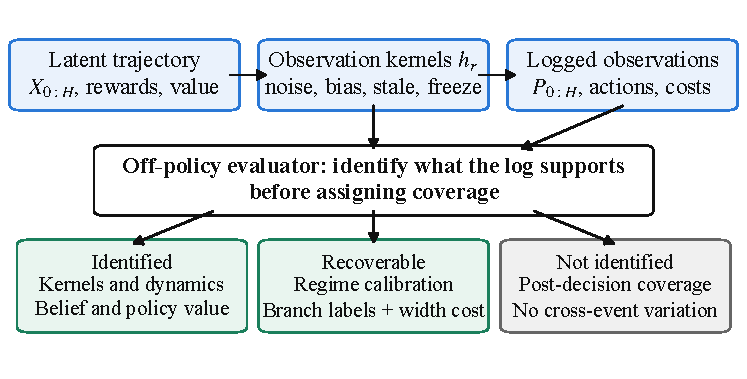
\includegraphics[width=0.55\linewidth]{../../figures/scis/fig0-observation-boundary.pdf}
\caption{Regime-dependent observation and the resulting identification and coverage boundary map. The evaluator reads the logged observations through the observation model and separates recoverable calibration from information that must be supplied additionally.}
\label{fig:0}
\end{figure}

A sensor that is accurate during normal operation, biased in a degraded mode, and frozen during an outage provides one example. Tokenized-equity automated market makers (AMMs) provide another: the reference market closes at night, on weekends, and on holidays, while the pool remains open. Its price is noisy during open hours, persistently biased during extended hours, stale during a freeze, and fixed during a halt. A policy evaluated on logged pool prices is therefore evaluated through a moving observation map. The AMM environment is used as a testbed; it is not the source of the methodological claim.

Two standard assumptions fail together. Calibration rows from different regimes are not exchangeable, and treating the observed price as the latent state misspecifies the model. The reward compounds the problem when it contains an unobserved path functional: importance-sampling and doubly robust (IPS/DR) estimators can reweight observed rewards but cannot reconstruct that term. Evaluation is therefore both partially observed and model-based.

Four lines of work frame this distinction: POMDP OPE \cite{shi2022,uehara2023,zhang2024,zhang2025,luo2026}, non-exchangeable conformal analysis \cite{barber2023}, pre-decision Mondrian calibration \cite{vovk2005,lei2018}, and conditional or selection-conditional coverage \cite{barber2021,jin2024jomi,lakkaraju2017}. Their combination leaves three missing objects: a regime-varying measurement kernel, an unobserved path-functional reward, and a branch label revealed only after the interval-forming decision.

We ask three questions. \textbf{Q1}: what is identifiable from logged observations under a regime-dependent observation model? \textbf{Q2}: when do standard OPE and conformal intervals fail, and when does calibration recover coverage? \textbf{Q3}: which coverage targets and policy values remain information-theoretically impossible or unidentifiable, even with unlimited data and a correctly specified model class?

We make three contributions.

\begin{enumerate}
\item \textbf{Post-decision coverage limits and recovery.} Theorem 3 proves that marginal coverage does not identify post-decision branch-conditional coverage for branch-blind, nondegenerate score rules and characterizes the sharp bound. Proposition 2 shows that calibration-side branch labels restore branch coverage at a width price. Theorem 2 supplies the supporting drift-aware marginal bound as a sup-CDF specialization of \cite{barber2023}.
\item \textbf{Observation-channel identification and its limits.} We formalize regime-dependent observation as a partially observed Markov decision process (POMDP) with an unobserved path-functional reward. Theorem 1 identifies the observation kernels, short-range dynamics, belief, and value $V^\pi$ under explicit assumptions and yields a consistent model-based plug-in. Theorem 4 proves within-class non-identification for a non-Markov freeze bridge without cross-event variation when endpoints do not determine the bridge reward.
\item \textbf{A reusable audit, evaluated across environments.} Protocol 1 turns this map into a four-step report of support, observation-map uncertainty, coverage/width, and identification status. Controlled experiments evaluate the audit at row, trajectory, branch, and identification levels, with stress and misspecification suites separating recoverable calibration from missing information. A second synthetic sensor-control environment tests the branch gap and recovery outside the AMM testbed. A post-hoc real-path replay on 33 events over 16 freeze episodes illustrates the audit as a calibration-window diagnostic.
\end{enumerate}

The following comparison isolates the methodological gap. Each entry is a boundary of the corresponding literature for our setting, not a claim that prior work lacks its own guarantees.

\vspace{4pt}
\noindent\begin{minipage}{\linewidth}\footnotesize\textbf{Table 1 Methodological positioning under regime-dependent observation}\par

\begin{tabular}{@{}>{\raggedright\arraybackslash}p{0.284\linewidth}@{\hspace{0.3em}}>{\raggedright\arraybackslash}p{0.180\linewidth}@{\hspace{0.3em}}>{\raggedright\arraybackslash}p{0.189\linewidth}@{\hspace{0.3em}}>{\raggedright\arraybackslash}p{0.247\linewidth}@{}}
\toprule
Line of work & Missing object for our setting & Limitation under regime-dependent observation & Our addition \\
\midrule
POMDP OPE \cite{shi2022,uehara2023,zhang2024,zhang2025,luo2026} & Regime-indexed kernels and latent path rewards & Bridge/revealing conditions do not characterize branch coverage & Parametric identification and a within-class boundary; model-based estimation is not unique in principle \\
Non-exchangeable conformal analysis \cite{barber2023} & Observation-kernel shift and information available only after a decision & Calibration shift alone does not characterize post-decision branch coverage & A sharp branch-conditional impossibility bound and a drift-aware supporting bound \\
Group or Mondrian calibration \cite{vovk2005,lei2018} & Labels that are unavailable before the prediction or decision & Pre-decision strata cannot isolate the post-decision branch & Calibration-side branch labels recover coverage with an explicit width cost \\
Conditional/selection-conditional coverage and selective labels \cite{barber2021,jin2024jomi,lakkaraju2017} & Regime-dependent OPE with latent path rewards & Selection/reference-set conditions differ from post-decision timing & Cross-level experiments and the audit \\
\bottomrule
\end{tabular}\end{minipage}

The central distinction is between calibration support and information availability. Evaluation-regime calibration restores full-window marginal coverage. Leave-one-regime-out calibration leaves EXTENDED a hard boundary: recovery requires evaluation-regime calibration data, not a better score. In the Wide $\tau=2$ event study, the marginal pipeline covers the post-rebalance branch at 0.667 and the hold branch at 0.971. The branch-union threshold built from calibration-side branch labels raises post-rebalance coverage to 0.958 at $3.97\times$ width. Pre-decision Mondrian cannot substitute for these labels because the branch label is not in the pre-decision $\sigma$-field. The second sensor-control environment reproduces the same gap and recovery, providing cross-environment confirmation of the branch gap and recovery.

The controlled environments hold selected latent laws fixed and use heuristic logging policies; the real-path case evaluates the protocol on observed paths through a post-hoc, regime-conditional usage check. The evidence therefore separates structural identification and coverage claims from live-market magnitudes.

\section{General setting and estimand}

We consider a partially observed Markov decision process whose observation kernel is indexed by an exogenous regime. The latent state evolves under a controlled transition law, while the log contains only regime-dependent observations, actions, and measured costs. The target is the value of a fixed target policy under this observation channel. The tokenized-equity AMM below is one instantiation of the general model; the sensor-control environment in \S6 provides another.

\subsection{Latent state and exogenous regimes}

In the AMM instantiation, the latent reference price is observed through a calendar-regime kernel: the pool price can be a noisy, biased, stale, or frozen transformation of that reference price. Time is discrete, $t=0,\dots,H$ ($H=336$ hourly steps in the environment). The latent state is $X_t=(S_t,Z_t)$, with $S_t>0$ the latent reference price and $Z_t$ the bias state, stale anchor, position, and cash. The latent price follows

\[
\begin{aligned}
\log S_{t+1}&=\log S_t+\kappa(\mu_{\log}-\log S_t)+\sigma\xi_t+J_t,\\
J_t&\sim N(0,(3\sigma)^2)\ \text{w.p. }0.005,\ \text{else }0,
\end{aligned}
\]

with one $\sigma$ per path. Regimes do not change the law of $S$ (I1$'$).

The calendar regime $r_t\in\mathcal R=\{\mathrm{OPEN},\mathrm{EXTENDED},\mathrm{WEEKEND},\mathrm{HOLIDAY},\mathrm{HALT}\}$ is known at $t$ and exogenous (A5): it is determined by the calendar, not by $S_t$ or the action. Transitions and observations are $X_{t+1}\sim T_{r_t}(\cdot\mid X_t,a_t)$ and $P_t\sim h_{r_t}(\cdot\mid X_t)$.

\subsection{Regime-dependent observation kernels}

Only OPEN anchors the current latent price; frozen regimes carry no current-$S$ information.

\vspace{4pt}
\noindent\begin{minipage}{\linewidth}\footnotesize\textbf{Table 2 Regime-dependent observation kernels and current-state information}\par

\begin{tabular}{@{}>{\raggedright\arraybackslash}p{0.179\linewidth}@{\hspace{0.3em}}>{\raggedright\arraybackslash}p{0.427\linewidth}@{\hspace{0.3em}}>{\raggedright\arraybackslash}p{0.293\linewidth}@{}}
\toprule
Regime & $h_r$ & Information about $S_t$ \\
\midrule
OPEN & $P_t=S_t e^{\varepsilon_t}$, $\varepsilon_t\sim N(0,\sigma_o^2)$ i.i.d. & noisy direct \\
EXTENDED & $P_t=S_t e^{\eta_t}$, $\eta_u=\phi_{\mathrm{ext}}\eta_{u-1}+N(0,\sigma_{\mathrm{ext}}^2)$, reset at OPEN & informative, block AR(1) bias \\
WEEKEND / HOLIDAY & $P_t=S_{\mathrm{last\,open},t}e^{\eta_t}$, $\eta_u=\phi_{\mathrm{stale}}\eta_{u-1}+N(0,\sigma_{\mathrm{stale}}^2)$ & stale anchor; no current $S$ \\
HALT & $P_t=P_{t-1}$ & none \\
\bottomrule
\end{tabular}\end{minipage}

The bias is not stationary inside a window: it is reset at every OPEN step and recurses only inside a non-OPEN block. Treating a frozen $P_t$ as a noisy proxy for $S_t$ is therefore misspecified.

\subsection{Actions, rewards, and value}

The LP chooses hold, rebalance, exit, or enter. The reward is

\[
R_t=\rho(X_t,a_t,X_{t+1})=\frac{\text{fees}_t+\Delta\mathrm{IL}^{\mathrm{true}}_t-\text{cost}_t}{V_0},
\]

where $\Delta\mathrm{IL}^{\mathrm{true}}_t$ is computed from the latent price path and the position and is not observed in logged data. This is why a purely importance-weighted estimator is unavailable: IPS/DR can reweight only observed rewards, and the target reward contains an unobserved path functional (\S3.4).

The target policy $\pi(a_t\mid H_t^o)$ is known, with $H_t^o=(P_{0:t},r_{0:t},a_{0:t-1},\text{position/cash})$; the logging policy $\mu$ is known or estimable. For $R_{\mathrm{eval}}\subseteq\mathcal R$ fixed by the calendar,

\[
\begin{aligned}
V^\pi(R_{\mathrm{eval}})&=\mathbb E_{\theta,\pi}\Bigl[\sum_{t:r_t\in R_{\mathrm{eval}}}\gamma^t\rho(X_t,A_t,X_{t+1})\Bigr],\\
\theta&=(T,h,\nu,\rho),
\end{aligned}
\]

with $\gamma\in(0,1]$; the full-window value takes $R_{\mathrm{eval}}=\mathcal R$. We write $G$ for the trajectory return and $G_r$ for its per-regime segment.

\subsection{Data and estimand}

The offline data are trajectories generated by $\mu$, with pool prices, regimes, actions, positions, cash, fees, and costs. The target is $V^\pi(R_{\mathrm{eval}})$; the conformal object in \S4 is the trajectory return $G$ (or $G_r$), not a per-row reward. The synthetic environment gives access to $S_t$ for validation, but no estimator below uses it.

Regimes are observed calendar labels rather than latent states; the identification analysis below does not estimate the kernels from real data.

\section{Identification}\label{sec:identification}

Under I1$'$, I2, I3, and the auxiliary conditions, the calendar-regime POMDP is identified from logged pool prices, and $V^\pi$ is a continuous functional of the identified components; cross-event variation (I5/I5$'$) is needed only when the freeze-period bridge is non-Markov.

\subsection{Assumptions}

Full assumptions, including T1--T4, are in Appendix A.1 of the Supplementary Material; we state only those that carry the argument.

\begin{itemize}
\item \textbf{I1$'$ (shared dynamics and cost).} Across regimes the $S$-component of $T_r$ and $\rho$ are shared (or share parameters in a known family); regimes change only $h_r$, the bias state, and OPEN anchoring, not volatility, jumps, or mean reversion.
\item \textbf{I2 (OPEN anchoring).} On OPEN, $P_t=S_t\exp(\varepsilon_t)$ with $\varepsilon_t\sim N(0,\sigma_o^2)$ i.i.d. and independent of $S$, actions, and bias; scale is normalized to one. What is identified is $\mathcal L(S_t\mid H_t^o)$, not $S_t$ pointwise.
\item \textbf{I3 (parametric observation family).} $h_r=h_{\theta_r}$ with finite-dimensional $\theta_r$; $\theta_r\mapsto\mathcal L(P\mid X,r)$ is injective; the bias is AR(1) with $|\phi_r|<1$, reset at OPEN and carried within non-OPEN blocks; innovations are independent of $S$, actions, OPEN noise, and independent across blocks.
\item \textbf{I5 (cross-event variation; non-Markov branch only).} Freeze event $e$ has endpoints $t_e^-,t_e^+$, duration $\tau_e$, and pre-freeze volatility $\sigma_e$. $Q^{\mathrm{end}}_{\tau,\sigma}$ is common across events, and the support of $(\tau,\sigma)$ contains a neighborhood of the target (or the target in its discrete support). Given $S_{t_e^-}=s^-$, event selection is conditionally independent of freeze innovations (A5).
\item \textbf{I5$'$ (bridge condition; non-Markov branch only).} If $T$ is not Markov on the freeze span, $Q^{\mathrm{path}}$ is identified only under (a) a parametric bridge family pinned down by endpoints and event data, or (b) direct path identification assumed; endpoints alone do not identify a path-dependent reward.
\end{itemize}

Auxiliary conditions: A1 bounded reward, A2 known target policy, A4 TV-kernel continuity, A5 exogenous calendar, A6 initial distribution, A7 no market impact, T1 anchor-parameter identifiability, T4 reward observability; A3$'$ (model-based support) only when $T$ depends on actions and $\pi$ selects actions with no logging support. Standard OPE overlap A3 is \textbf{not} used: there is no importance-weight representation of the target reward.

I5/I5$'$ appear only in Theorem 1(c)(ii); the experimental environment is the Markov branch, where they are redundant. T1 is an identification condition, not a conclusion: the theorem is parametric.

\subsection{Theorem 1 (identification)}

\textbf{Theorem 1 (Identification under regime-dependent observation).} Assume I1$'$, I2, I3, A1, A2, A4--A7, T1, T4, and A3$'$ whenever $T$ depends on actions and $\pi$ selects actions with no logging support. In part (c)(ii), additionally assume I5, I5$'$, T2, T3. Then:

\textbf{(a) Anchor observation.} $h_{\mathrm{OPEN}}$ is identified: $\sigma_o$ and $\mathcal L(S_t\mid H_t^o)$ on OPEN histories are identified; $P_t$ is a noisy measurement of $S_t$, and $S_t$ is not pointwise identified.

\textbf{(b) Short-range dynamics.} The $S$-component and EXTENDED bias component of $T$ are identified from calendar-adjacent OPEN and EXTENDED observations. Other bias components are completed in (d); the joint kernel is not claimed before (d).

\textbf{(c) Freeze-period bridge.} Two branches:

(i) \textbf{Markov branch (the experimental environment).} If $T$ is Markov on the freeze horizon and its $S$-component is identified as in (b), then for every $\tau$ the path law $Q^{\mathrm{path}}_{\tau,\sigma}(\cdot\mid s^-)$ is the $\tau$-step composition of that component started at $s^-$; no I5/I5$'$, T2, T3, or support restriction is needed.

(ii) \textbf{Non-Markov branch.} If $T$ is not Markov, then under I5, T2, and T3 the endpoint law $Q^{\mathrm{end}}_{\tau,\sigma}(\cdot\mid s^-)$ is identified for $\Pi$-a.e. $s^-$, with errors-in-variables and regime-specific endpoint noise $h_{r(t_e^-)}$, $h_{r(t_e^+)}$. $Q^{\mathrm{path}}$ needs the additional I5$'$; endpoints alone do not identify path-dependent rewards.

\textbf{(d) POMDP components.} The remaining regime-specific bias components of $T$, all kernels $h_r$, $\nu$, and $\rho$ (using T4 and A7) are identified; hence the belief $b_t(\cdot)=\mathbb P(X_t\in\cdot\mid H_t^o)$ is identified for every observable history.

\textbf{(e) Value and plug-in.} For any known target policy $\pi$ satisfying A2 and A3$'$, $V^\pi(R_{\mathrm{eval}})$ is identified. If $\hat\theta\to\theta$ in the TV-kernel topology of A4, the plug-in $\hat V^\pi=V^\pi(\hat\theta)$ is consistent: $\hat V^\pi\to V^\pi(\theta)$ in probability (or a.s., according to the mode of $\hat\theta\to\theta$).

The proof chain has four lemmas: Lemma 1 gives (a)--(b) for the OPEN and EXTENDED components; Lemma 2 gives (c)(ii), while in branch (i) (c) follows from Lemma 1 plus Markov composition; Lemma 3 gives (d) and the cross-regime belief; Lemma 4 gives (e). Appendix A.1 gives the derivations under their stated conditions (the known-start linear-Gaussian/no-jump case; T1 is assumed for the jump family), and the complete history-conditional belief across regimes is obtained after Lemma 3, not from OPEN data alone.

\subsection{Proof chain}

The proof has four moves. Repeated OPEN observations identify $\sigma_o$ and $\mathcal L(S_t\mid H_t^o)$ as a noisy measurement, not $S_t$ pointwise. Calendar-adjacent OPEN and OPEN--EXTENDED pairs then identify the $S$-component and EXTENDED bias using within-block $u$-profiles $(1-\phi_r^{2u})$, never crossing a closed regime. The freeze path is the $\tau$-step composition in the Markov branch; in the non-Markov branch the endpoint law needs the errors-in-variables deconvolution under I5/T2/T3 and the path law needs I5$'$, so ``endpoint identified'' is not upgraded to ``path identified.'' The remaining kernels, initial distribution, and reward complete the POMDP, and $V^\pi$ is a continuous functional of it in the TV topology, so the plug-in inherits consistency. No finite-sample rate is claimed: TV continuity is a population statement, and the deconvolution is ill-posed in the nonparametric version we do not claim.

\subsection{Why model-based, and what replaces a uniform value-error bound}

\textbf{Why not standard observed-reward IPS/DR.} The reward contains $\Delta\mathrm{IL}^{\mathrm{true}}$, a function of the latent path and position. Logs observe fees and costs but not this functional, which standard IPS/DR cannot manufacture. Overlap A3 belongs to the variant with a known observable reward, not to this estimand. Bridge-function and future-dependent value methods are alternatives under their own existence, completeness/revealing, proxy, and overlap conditions; model-based estimation is not unique in principle. Theorem 4 nevertheless gives observationally equivalent models whose bridge rewards no future or history proxy can distinguish. We use a parametric model-based route.

\textbf{Proposition 1 (No single uniform value-error bound).} A single $W_1$ or Le Cam bound does not give a uniform value-error bound for a fixed policy. We therefore report a \textbf{decomposition}, not a theorem: (a) a $W_1$ estimation term, (b) a predictive-distribution TV information term, and (c) a policy boundary/action-flip diagnostic. Under the regularity conditions of Appendix A.2 (finite policy-variation constant and controlled $W_1$), (a)--(b) have a provable mixed bound; (c) is a diagnostic refinement for observable policies. Under one-sided drift the state-level TV bound can be empty: OPEN and WEEKEND kernels can have TV near one when $S_t$ is far from the stale anchor. We report the three terms separately in Appendix Table B1 and \S7.9 and do not compress them into a single $\kappa_{\mathrm{obs}}$.

The state-level TV sensitivity (Proposition A.1 in Appendix A.2) is only a worst-case sensitivity; the formal guarantees are Theorems 1 and 2, not a uniform value-error bound.

\subsection{What identification does not give}

Theorem 1 does \textbf{not} give pointwise identification of $S_t$, nonparametric identification, the full freeze path without I5$'$, a finite-sample rate, or a general necessity claim for I5 (Theorem 4 is a within-class existence result). Its empirical check is synthetic and regimes are calendar-exogenous; a price-triggered halt violates A5.

\section{Estimation and coverage}

A model-based plug-in estimator, combined with split conformal on trajectory-level scores and a drift-aware finite-sample correction, gives valid \textbf{marginal} coverage when calibration data exist in the evaluation regime; the correction does not upgrade to branch-conditional coverage.

\subsection{The G0 pipeline}

The pipeline estimates an errors-in-variables-corrected OPEN anchor; $\kappa,\mu,\text{jump}$; the kernels $h_r$; and a per-path $\sigma$. In the controlled environment it recovers $\sigma_o=0.000496$ (target $0.0005$), $\kappa_{\mathrm{mr}}=0.00285$ (SE $0.00074$), and freeze-condition slopes $0.977$ at $\tau=2$ and $0.741$ at $\tau=81$ (targets $0.991$ and $0.782$); these validate the synthetic environment, not real data.

\subsection{Trajectory-level split conformal}

The conformal object is $G$ or $G_r$, not a per-row reward. We use \textbf{leave-fold-out split conformal}, not CV+: for each fold $f$, $\hat q$ is the $k$-th order statistic of the other four folds' scores, and coverage is declared when the held-out score is at most $\hat q$. For the 128-path L2 and Theorem 2 illustration, folds have sizes $28/28/24/24/24$, so $n_{\mathrm{cal}}\in\{100,104\}$ and $k\in\{91,95\}$ at $\alpha=0.1$. The larger L1 calibration and evaluation sets are described separately in \S6.2. This is one split per test point; 2A applies per fold if scores within a $\tau$ are i.i.d. (the four windows of a seed share a fold, so calibration and test use different seeds). We report raw, studentized, and CQR scores, with within-regime calibration when available and LORO otherwise.

\subsection{Drift-aware finite-sample coverage (Theorem 2)}

The finite-sample bound specializes the non-exchangeability framework of \cite{barber2023} to a sup-CDF drift; the estimated-$\kappa$ PAC form and the four-object separation below are the additions here.

Let $E_1,\dots,E_n$ be i.i.d. $F_{\mathrm{cal}}$, set $k=\lceil(n+1)(1-\alpha)\rceil$, let $\hat q=E_{(k)}$ ($\hat q=\infty$ if $k>n$), and define

\[
\kappa=\sup_x|F_{\mathrm{cal}}(x)-F_{\mathrm{test}}(x)|,
\quad
\hat\kappa=\sup_x|\hat F_{\mathrm{cal}}(x)-\hat F_{\mathrm{test}}(x)|.
\]

\textbf{Theorem 2A.} If a test score $E\sim F_{\mathrm{test}}$ is independent of the calibration sample, then for $k\le n$,

\[
\Pr\{E\le\hat q\}\ge\max\Bigl(0,\frac{k}{n+1}-\kappa\Bigr)\ge\max(0,1-\alpha-\kappa),
\]

with an exact finite-sample marginal lower bound for known $\kappa$; if $k>n$, $\hat q=\infty$ and coverage is $1$.

\textbf{Theorem 2B.} If, in addition, $E'_1,\dots,E'_m$ are i.i.d. $F_{\mathrm{test}}$, independent of the calibration sample and of $E$, then with probability at least $1-\delta_{\mathrm{cal}}-\delta_\kappa$,

\[
\begin{aligned}
F_{\mathrm{test}}(\hat q)&\ge\max\Bigl(0,\frac{k}{n}-\varepsilon_{\mathrm{cal}}-\hat\kappa-\varepsilon_\kappa\Bigr),\\
\varepsilon_{\mathrm{cal}}&=\sqrt{\frac{\ln(2/\delta_{\mathrm{cal}})}{2n}},\\
\varepsilon_\kappa&=\sqrt{\frac{\ln(4/\delta_\kappa)}{2n}}+\sqrt{\frac{\ln(4/\delta_\kappa)}{2m}},
\end{aligned}
\]

a PAC conditional-coverage bound given the data.

\textbf{Corollary 2.2.} Let $\gamma=\Pr\{E\le\hat q\}$, a constant given the distributions and $n,k$. With $\hat\kappa$ and $\varepsilon_\kappa$ as above, with probability at least $1-\delta_\kappa$,

\[
\gamma\ge\max\Bigl(0,\frac{k}{n+1}-\hat\kappa-\varepsilon_\kappa\Bigr).
\]

This bounds the marginal coverage rate, not the realized interval.

The plug-in $\max(0,1-\alpha-\hat\kappa)$ is a point estimate, not a guarantee: 2A, 2B, Corollary 2.2, and Remark 2.3's expectation bound are four distinct objects; 2B does not imply a marginal bound of the same value, and Corollary 2.2 does not give conditional coverage.

At $n=m=128$ and $\alpha=0.1$, the 95\%-confidence bounds are:

\vspace{4pt}
\noindent\begin{minipage}{\linewidth}\footnotesize\textbf{Table 3 Finite-sample coverage bounds at $n=m=128$ and $\alpha=0.1$}\par

\begin{tabular}{@{}>{\raggedright\arraybackslash}p{0.174\linewidth}@{\hspace{0.3em}}>{\raggedleft\arraybackslash}p{0.159\linewidth}@{\hspace{0.3em}}>{\raggedleft\arraybackslash}p{0.164\linewidth}@{\hspace{0.3em}}>{\raggedleft\arraybackslash}p{0.178\linewidth}@{\hspace{0.3em}}>{\raggedleft\arraybackslash}p{0.225\linewidth}@{}}
\toprule
Score & $\hat\kappa$ (Wide / Narrow) & plug-in (Wide / Narrow) & 2B (Wide / Narrow) & Cor 2.2 (Wide / Narrow) \\
\midrule
raw & 0.8594 / 0.8750 & 0.0406 / 0.0250 & 0 / 0 (empty) & 0 / 0 (empty) \\
studentized & 0.1172 / 0.2344 & 0.7828 / 0.6656 & 0.3844 / 0.2673 & 0.5281 / 0.4109 \\
CQR & 0.5781 / 0.6172 & 0.3219 / 0.2828 & 0 / 0 (empty) & 0.0672 / 0.0281 \\
\bottomrule
\end{tabular}\end{minipage}

\noindent{\footnotesize\textbf{Notes.} 95\% denotes the bound's confidence level; $\alpha=0.1$ is nominal miscoverage. Per-fold 2A with plugged-in $\hat\kappa$ is $0.784$--$0.788$ (a point estimate). With a strict per-fold $\hat\kappa$ ($m=24$--$28$), the bounds weaken sharply: 2A is $0.552$--$0.783$, 2B is $0.000$--$0.165$ (empty in one of five folds, where $\hat\kappa=0.353$), and Corollary 2.2 is $0.105$--$0.336$. Replacing only $m$ while keeping the pooled $\hat\kappa$ gives $0.170$--$0.184$, a mixed plug-in that is not a strict per-fold calculation. The per-fold values are reported in Appendix A.3, Table A2. Both variants estimate $\hat\kappa$ from the evaluated test fold, so they are in-sample diagnostics, not independent checks of the 95\% PAC frequency; five correlated folds from one dataset cannot validate it either.\par}

\textbf{Independent three-sample check.} In 100 replicates, calibration and drift estimation never touch the final test. Studentized coverage is 0.906--0.910; raw gives 0.105 forward and 1.000 reverse at 18.7$\times$ width, and CQR has nearly empty bounds (Appendix Table A3).

\subsection{Observable-$h$ estimation}

A state-space Gaussian-sum filter with trimmed likelihood and a $|z|>3$ mask estimates $h$ without the latent $S$ path; \S7.5 reports the parameter estimates and coverage sensitivity across five specifications. Theorem 1(e) assumes sup-TV convergence of every component of $h$. The observable-only pipeline does not satisfy that premise for \texttt{open\_sd} and \texttt{ext\_phi}, which are weakly identified in this design rather than non-identifiable in population. Its coverage stability is therefore an empirical robustness result, not a corollary of Theorem 1(e).

\subsection{Reproduction}

Table and figure inputs, generation scripts, seeds, folds, and derived-value checks are listed in Appendix C. These checks support the marginal and trajectory-level statements above; they do not turn Theorem 2B into conditional coverage, the plug-in into a calibrated interval, or one dataset into a PAC-frequency validation, and they do not supply branch-conditional coverage.

\section{Impossibility boundaries}

Regime shift, post-decision branch conditioning, and weak identification of the observation kernel are independent axes of failure; none repairs another. Within the non-Markov freeze class and with a bridge reward not determined by endpoints, there exist observationally equivalent models with different values (Theorem 4). No calibration trick substitutes for the missing information.

\subsection{Marginal coverage does not identify branch coverage (Theorem 3)}

Let $X$ be the pre-decision covariate, $Y$ the return, and $B\in\{0,1\}$ a \textbf{post-decision branch} (e.g., rebalance vs hold), observed at evaluation but unavailable when the interval is formed. Set $q_b(x)=\Pr(B=b\mid X=x)$, $q_b=\Pr(B=b)$, $\alpha(x)=\Pr(Y\notin C(x)\mid X=x)$, $\alpha=\mathbb E[\alpha(X)]$, and $\mathrm{cov}_b(C)=1-\mathbb E[f_b(X)]/q_b$, where $f_b(x)=\Pr(Y\notin C(x),B=b\mid X=x)$.

\textbf{Theorem 3 (branch impossibility; finite-sample form in Appendix A.4).}

\textbf{(a) Trivial bound.} For any $C$ with marginal miscoverage $\alpha$ and $q_b>0$,

\[
\mathrm{cov}_b(C)\ge1-\frac{\alpha}{q_b}.
\]

If $C$ is branch-blind, the stronger bound is

\[
\mathrm{cov}_b(C)\ge1-\frac{\mathbb E[\min(\alpha(X),q_b(X))]}{q_b}\ge1-\frac{\alpha}{q_b}.
\]

\textbf{(b) Non-identification.} Fix the law of $(X,Y)$ and $q_b(x)\in(0,1)$. Let $C_n$ be any branch-blind score rule with a possibly data-dependent threshold, and suppose

\[
\Pr_{D_n}\Bigl(\Pr_X\bigl(0<\alpha_{D_n}(X)<1\bigr)>0\Bigr)>0,
\]

where $\alpha_{D_n}(x)=\Pr(Y\notin C_n(x)\mid X=x,D_n)$. Then two joint laws of $(X,Y,B)$ share $(X,Y)$ and $q_b(x)$ but differ in branch-$b$ coverage; they differ only in the coupling $B\mid(X,Y)$, invisible to pre-decision data. The non-degenerate gap is

\[
\frac{\mathbb E[\min(\alpha(X),q_b(X))-\max(0,\alpha(X)+q_b(X)-1)]}{q_b}>0.
\]

\textbf{(c) Sharp bound and minimax.} For a fixed branch-blind score rule, the sharp bound over compatible couplings is $1-\mathbb E[\min(\alpha(X),q_b(X))]/q_b$. Within branch-blind score rules with $\mathbb E[\alpha(X)]=\alpha$ and $\alpha(X)\le q_b(X)$ a.s., when this class is nonempty and $q_b>0$, the minimax value is exactly $1-\alpha/q_b$. Under the non-atomic conditional-law condition ($Y\mid X=x$ non-atomic for almost every $x$), the class is nonempty exactly when $q_b\ge\alpha$; Appendix A.4 constructs a conditional-CDF score with threshold one and failure function $\alpha(x)=(\alpha/q_b)q_b(x)$. Outside this class the sharp value can be higher, so the trivial bound may be loose. Finite-sample versions are Theorems 3A--3C in Appendix A.4.

\textbf{Interpretation.} Marginal coverage is a mixture over branches; a small-$q_b$ branch can absorb a large conditional failure rate while the marginal rate stays $\alpha$. Pre-decision Mondrian cannot isolate a post-decision branch whose label is unavailable at prediction time: an information limit, not an algorithmic defect.

\subsection{The price of branch-wise calibration (Proposition 2)}

If branch labels are available in calibration, branch-wise split conformal restores branch coverage.

\textbf{Proposition 2 (branch-wise calibration and its price; finite-sample form in Appendix A.5).}

\textbf{(a) Branch-wise coverage.} Suppose calibration and test points are exchangeable, and the pairs $(X_i,Y_i)$ are exchangeable within each branch $b$. Let $n_b=\#\{i\le n:B_i=b\}$, $k_b=\lceil(n_b+1)(1-\alpha)\rceil$, and $\hat q_b$ be the $k_b$-th order statistic of branch-$b$ scores ($\hat q_b=\infty$ if $k_b>n_b$). Then $\Pr(Y\in C_b(X)\mid B=b)\ge1-\alpha$ and $\Pr(Y\in C_\cup(X)\mid B=b)\ge1-\alpha$, where $C_\cup=C_0\cup C_1$; CQR uses the convex hull of the union.

\textbf{(b) Coverage dominance.} With $\hat q$ the marginal threshold and $\hat Q=\max(\hat q_0,\hat q_1)$, any calibration set (including ties and empty branches) gives $\hat Q\ge\hat q$. For a common scalar score the set $\{y:s(x,y)\le\hat Q\}$ is exactly $C_0(x)\cup C_1(x)$, so the raw union contains the marginal set; for CQR the union is an interval and equals its convex hull. For a general non-interval score dominance holds for the convex hull of the union, and if the branches use different score functions raw-union dominance must be checked separately. The price is weakly larger width.

\textbf{(c) No distribution-free gain per unit width.} Fix a calibration set with $\hat Q>\hat q$. For any $m\ge1$ and positive $g(\Delta w)$, some test distribution gives zero branch-$b$ coverage gain while $\Delta w=2(\hat Q-\hat q)$ (or the CQR analog) is strictly positive; hence no distribution-free bound ``coverage gain $\ge g(\Delta w)$'' holds.

\textbf{Interpretation.} Branch-wise calibration buys branch coverage with width; the gain depends on the target distribution, and branch-union is not claimed optimal ($\hat Q$ is sufficient, not an optimizer). The within-$\tau$ width ratio is $1.03$--$3.97$ across the 12 identified within-$\tau$ cells (two policies $\times$ three scores $\times$ two directions), with small branches noise-dominated. Across the 56 branch-union blocks (112 branch cells), every branch had a nonempty calibration set, no threshold was infinite, and the smallest branch calibration count was 16.

\subsection{Cross-event variation is substantive (Theorem 4)}

Within the model class below, there are observationally equivalent models with different values.

\textbf{Theorem 4 (within-class non-identification without I5/I5$'$; finite-sample two-point bound in Appendix A.6).} Consider the class of models with unobserved freeze interiors, only OPEN data and noisy endpoints, and common open-period dynamics, observation kernel, endpoint noise, and calendar. Suppose the reward's bridge expectation is not determined by endpoints: two bridge laws $Q_1,Q_2$ have the same endpoints and observable law but $\mathbb E_{Q_1}[\rho]\ne\mathbb E_{Q_2}[\rho]$. Then there exist two models $P,Q$ in this class, independent of $n$ and $\hat V_n$, such that for every $n$ and every observable-data estimator $\hat V_n$ (possibly randomized externally): (i) the observable-data laws are identical under $P$ and $Q$; (ii) $|V^\pi(P)-V^\pi(Q)|=\Delta>0$; and (iii) $\max(\mathbb E_P|\hat V_n-V^\pi(P)|,\mathbb E_Q|\hat V_n-V^\pi(Q)|)\ge\Delta/2$. The result is an existence statement inside this class. It does not assert that I5/I5$'$ are necessary for identification in every model, and it does not prove that the constructed models satisfy I1$'$.

The construction uses two Brownian bridges with the same endpoints and different volatilities, plus a reward with $-\lambda\,\mathrm{QV}_{\mathrm{freeze}}$; since $\mathbb E[\mathrm{QV}]=\sigma^2\tau$, the value gap is $\lambda\tau|\sigma'^2-\sigma^2|$. The bound is information-theoretic: no estimator is uniformly consistent over the class, though a particular plug-in may work on the observed data.

\textbf{Empirical correspondence.} The de-freeze-jump and bridge stresses in \S7.6 show the same direction: open-only calibration under-covers when a latent freeze-span variance component is active, while cross-event calibration recovers coverage. The same-endpoint diagnostic produces bit-identical observed pool prices under $\nu$ and $2\nu$ while the latent quadratic-variation ratio is $3.85$ against a theoretical $4$ (Appendix Table B2, Panel D). This is an empirical correspondence, not a test of I5 on real data; the main environment is the Markov branch, where I5 is redundant.

\subsection{Three independent axes}

The axes are not interchangeable.

\vspace{4pt}
\noindent\begin{minipage}{\linewidth}\footnotesize\textbf{Table 4 Three independent failure axes and their remedies}\par

\begin{tabular}{@{}>{\raggedright\arraybackslash}p{0.189\linewidth}@{\hspace{0.3em}}>{\raggedright\arraybackslash}p{0.219\linewidth}@{\hspace{0.3em}}>{\raggedright\arraybackslash}p{0.179\linewidth}@{\hspace{0.3em}}>{\raggedright\arraybackslash}p{0.174\linewidth}@{\hspace{0.3em}}>{\raggedright\arraybackslash}p{0.144\linewidth}@{}}
\toprule
Axis & What is missing & What fails & What can repair it & What cannot \\
\midrule
Regime shift & regime calibration data & marginal coverage under LORO, especially EXTENDED & within-regime calibration & marginal conformal on another regime \\
Branch conditioning & post-decision $B$ at prediction & branch-conditional coverage & branch-wise calibration with labels & pre-decision Mondrian alone \\
Observation kernel & strong identification of $h$ & precise $h$ estimates & more informative data or stronger priors & treating \texttt{h\_obs} as truth \\
\bottomrule
\end{tabular}\end{minipage}

The axes can co-occur, but fixing one does not fix another: regime-aware calibration does not recover branch-conditional coverage, and branch-wise calibration does not recover coverage in a regime with no calibration data. The third axis is empirical: \S7.5 separates weak identification of \texttt{open\_sd} and \texttt{ext\_phi} from the coverage sensitivity to those specifications.

\section{Experimental design}

\subsection{Environment and data}

The environment is a synthetic 24/7 tokenized-equity AMM. A latent reference price follows a mean-reverting log process with hourly volatility $\sigma=0.008\exp(N(0,0.35))$, mean reversion $\kappa=0.003$ toward $\mu=\log 100$, and a jump $N(0,(3\sigma)^2)$ with probability $0.005$ per hour. The pool price passes through a regime-dependent observation kernel: OPEN adds $N(0,0.0005^2)$; EXTENDED adds an AR(1) deviation with $\phi=0.8$ and sd 0.002; WEEKEND and HOLIDAY add an AR(1) deviation with $\phi=0.98$ and sd 0.0008 around the last open price; HALT freezes the pool price. The 14-day calendar has weekday OPEN 09:00--16:00, EXTENDED otherwise, a weekend freeze from Friday 16:00 to Monday 09:00, one holiday, and one two-hour halt.

The latent law is identical across regimes; only the observation kernel changes. This isolates observation-mapping drift from latent-dynamics drift, which is the object of this study, but real venues may change both at once. The LP owns a Uniswap-v3 range position (30 bp fee tier, 1\% in-range liquidity, 100,000 notional). Reward is fee income plus the change in fundamental IL minus rebalancing cost, normalized by notional. The logging dataset is 32 seeds $\times$ 4 windows $\times$ 6 heuristic policies $\times$ 336 hourly steps = 258,048 rows. The six policies are Passive Wide, Passive Narrow, Periodic 24h, Threshold 2\%, Exit Freeze 50, and Stochastic 5\%. The target policies Wide Rebalance 2\% and Narrow Rebalance 1\% are outside the logging set, so all target-policy values are model-based OPE. The environment is synthetic and the logging policies are heuristic, not trained RL; \S7.8 reports a post-hoc real-path case, while the synthetic environment remains the controlled identification study.

For the semi-synthetic calibration in \S7.7, one year of public hourly bars for SPY, QQQ, TSLA, and NVDA provides return-dynamics benchmarks, and measured Chainlink 24/5 stale intervals provide freeze-duration and reopen-gap benchmarks. These inputs calibrate marginal scales; they are not used as a paired pool-price/reference-price sample for independently fitting the full observation map. Appendix Table B3 reports the calibration and carries the synthetic observable-only $h$ estimate as a limitation.

\subsection{Protocols}

Each level isolates one design axis. L0 trains on a chronological 70\% of the rows from the other four regimes, calibrates on the remaining 30\%, and tests on all rows of a held-out regime, comparing pooled, Mondrian, similarity-class, and strategy-conditional radii against an i.i.d. split. L1 uses independent calibration and evaluation sets of 512 paths each (128 seeds $\times$ four windows per set), distinct from the 32-seed logging panel and the 128-path L2 event study. We use split conformal at $\alpha=0.1$, raw/studentized/CQR scores and a Gaussian plug-in, under within-window, within-regime, leave-one-window-out, and leave-one-regime-out protocols; the paired bootstrap resamples test paths 2,000 times. L2 is a freeze-to-OPEN event study at $\tau=2$ (main) and $\tau=81$ (transfer), with five-fold out-of-fold predictions by path and branch thresholds computed on the calibration side. L3 varies trimming and volatility source across five observation-map specifications. The I5 stress suite has two variants: an unfreeze-jump variant that compares $\gamma_{\mathrm{st}}=4$ with a $\gamma_{\mathrm{st}}=0$ placebo, and a non-Markov bridge variant that replaces the freeze span with a Brownian bridge pinned at the latent endpoints and compares $\nu_{\rm mult}=0.6$ with a $\nu_{\rm mult}=0$ placebo. The separate misspecification protocol reruns the L1 comparison on a reduced seed set with the model side fixed at G0 while the data-generating process departs from the generating family in one ingredient at a time: AR(2) rather than AR(1) observation noise, Student-$t(3)$ rather than Gaussian jumps, 15\% regime-label noise, and a hidden stale observation state. Appendix Table B4 reports it. Full counts, hyperparameters, and the stress-variant formulas are in Appendix B.

The general sensor-POMDP has 48 linear-Gaussian control steps, eight logging burn-in steps, and normal, AR(1)-biased, and stale-observation regimes. The predictors share the known control coefficient $B=0.35$ and the identified-belief target-action rule/filter. The identified-transition predictor also knows $A$, $\sigma$, and the observation model; the fitted-transition comparator estimates only its rollout AR(1) coefficient and residual scale from burn-in data. This compares transition misspecification, not observation filters or joint estimation. The branch label records any target intervention of magnitude at least 0.65 and is used only for calibration-side thresholds and post-hoc coverage evaluation. Appendix B gives the full equations.

\subsection{Metrics and reporting conventions}

Coverage is the fraction of test units whose interval contains the realized reward. The aggregate gap is the test-weighted mean of $\max(0,0.9-\text{coverage})$ over dense regimes, so a zero is saturated and not by itself evidence of no under-coverage. Widths are mean interval widths; width ratios are union width over marginal width unless stated otherwise. Binomial standard errors treat rows or events as independent and are lower bounds. Paired comparisons use path-level bootstrap 95\% intervals. The nominal level is 90\% ($\alpha=0.1$); 95\% intervals are a separate object and are labeled as such. Branch cells with 24 events are read for direction only. Positive results are consistency checks within the same parameter family, not empirical superiority. The inline result summaries and Appendix Tables B1--B5/B7--B9 are generated by the scripts and inputs listed in Appendix C; Appendix Table B6 is hand-authored.

\section{Results}\label{sec:results}

We report results by research question. Unless stated otherwise, the nominal level is 90\% ($\alpha=0.1$), and intervals in brackets are 95\% confidence intervals for a coverage proportion, not prediction intervals. In every multi-series panel, colour is redundant with marker shape or line style, and the legend names each series.

\subsection{Row-level coverage (L0)}

A naive global split-conformal pipeline under-covers held-out WEEKEND at 0.8626 [0.8604, 0.8648], against 0.8997 for an i.i.d. random split. The gap persists across logging strategies and windows. A max fallback from the other regimes restores WEEKEND coverage to 0.9020 at 1.31$\times$ width; the stale similarity fallback gives 0.9033 for OPEN and 0.9055 for EXTENDED at 0.83$\times$ and 0.79$\times$.

The held-out regime contributes no calibration rows, so L0 is a fallback consistency check, not within-regime calibration or evidence of superiority. The harder failures occur at trajectory and branch levels. Figure~\ref{fig:3} reports the regime and strategy details.

\begin{figure}[!ht]
\centering
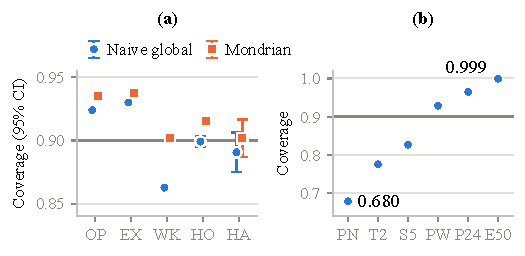
\includegraphics[width=0.55\linewidth]{../../figures/scis/fig3-l0-coverage.pdf}
\caption{Panel (a), held-out-regime row-level coverage for the naive global and Mondrian rules, with dots as point estimates and 95\% binomial whiskers. Panel (b) shows naive-global coverage across logging strategies only, with no Mondrian series and no whiskers. OP, EX, WK, HO, and HA abbreviate OPEN, EXTENDED, WEEKEND, HOLIDAY, and HALT; E50, PN, T2, S5, PW, and P24 abbreviate the six logging strategies (Exit Freeze 50, Passive Narrow, Threshold 2pct, Stochastic 5pct, Passive Wide, Periodic 24h). Nominal coverage is 90\% ($\alpha=0.1$).}
\label{fig:3}
\end{figure}

\subsection{Trajectory and regime coverage (L1)}

\textbf{Plug-in intervals.} The naive Gaussian full-window interval covers 0.666 (Wide) and 0.670 (Narrow), against nominal 0.90. The identified G0 pipeline improves this to 0.844/0.836, still below nominal. A correct conditional mean and model-based standard deviation therefore do not calibrate a path functional's tails.

\textbf{Recovery and hard boundaries.} Conformalizing the same predictions restores full-window within-window coverage to 0.895--0.930 and regime within-regime coverage to 0.892--0.908. Under leave-one-regime-out calibration, raw scores fall to 0.867--0.880; EXTENDED remains below nominal at 0.666--0.803 (studentized) and 0.576--0.740 (CQR), while width ratios stay near one. Evaluation-regime data, rather than a better score or wider interval, is the limiting resource.

Paired bootstrap intervals show no uniform conformal advantage for identified over naive pipelines: all full-window score differences include zero, although regime-level CQR differences are positive and plug-in differences are large. Thus identification helps the plug-in but adds little after conformalization. Figure~\ref{fig:4} reports the EXTENDED collapse and these comparisons.

\begin{figure}[!ht]
\centering
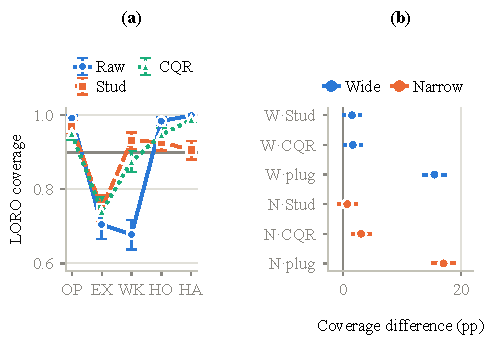
\includegraphics[width=0.55\linewidth]{../../figures/scis/fig4-l1-boundary.pdf}
\caption{Panel (a), leave-one-regime-out coverage for the Wide identified model by score; dots are point estimates and whiskers are 95\% binomial intervals. Panel (b), identified-minus-naive coverage differences in percentage points at the regime level with 95\% path-bootstrap intervals; W/N denote the Wide/Narrow policies and Stud, CQR, plug denote the studentized, CQR, and plug-in scores. OP, EX, WK, HO, and HA abbreviate OPEN, EXTENDED, WEEKEND, HOLIDAY, and HALT. Nominal coverage is 90\% ($\alpha=0.1$).}
\label{fig:4}
\end{figure}

\subsection{Post-decision branch coverage (L2)}

Branch conditioning is a separate axis. In the Wide $\tau=2$ event study, the marginal pipeline covers the hold branch at 0.971 ($n=104$) but the rebalance branch at 0.667 ($n=24$); overall marginal coverage is 0.914. The trivial bound at $\hat q_b=24/128$ and the measured overall coverage 0.914 is 0.542, so the observed branch coverage is above the worst-case floor but far below nominal.

The small-sample caveat is quantitative. Cell-wise Wilson 95\% intervals are [0.919, 0.990] on hold and [0.467, 0.820] on rebalance; the rebalance interval is 0.35 wide and lies entirely below 0.90. The deficit is directionally clear, but its magnitude is not pinned down; Appendix Table B12 (Panel D) reports all three scores.

The calibration-side branch-union threshold $\max(\hat q_{\rm hold},\hat q_{\rm rebalance})$ raises rebalance coverage to 0.958 for the studentized score (raw 0.917, CQR 0.917) and overall union coverage to 0.992, at overall width ratios 3.97$\times$, 3.96$\times$, and 3.37$\times$; the hold union is 1.000 in all three rows. At $n=24$ the studentized rebalance union interval [0.798, 0.993] contains 0.90, so union coverage is compatible with nominal but does not establish it. Union coverage dominates marginal coverage in 56/56 method-by-direction blocks and 112/112 cells; Appendix Table B12 (Panel B) reports the taxonomy, showing that branch-union often spends width on a branch that was already covered.

Pre-decision Mondrian cannot substitute for the post-decision label. Post-rebalance coverage under these two stratifications ranges from 0.583 to 0.708 across the 12 cells (three seeds, two scores, two stratifications), against 0.971 on hold and 0.667 on rebalance in the unstratified pipeline. The branch label is not in the pre-decision $\sigma$-field, exactly as Theorem 3 states.

Cross-event transfer is also only partial. Calibrating at $\tau=81$ and testing at $\tau=2$, Wide rebalance coverage moves from 0.667 to 0.750 (width 1.27$\times$, \texttt{ambiguous}) for the identified studentized score, and from 0.750 to 0.875 (width 1.67$\times$, \texttt{ambiguous}) for identified CQR. Branch-union helps, but it does not clear nominal when calibration and test event types differ. Figure~\ref{fig:5} shows the branch dots and the union-dominance scatter.

\begin{figure}[!ht]
\centering
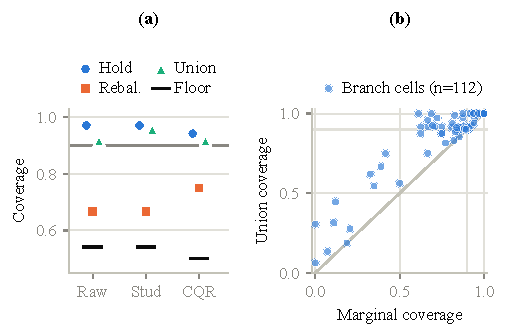
\includegraphics[width=0.55\linewidth]{../../figures/scis/fig5-l2-branches.pdf}
\caption{Panel (a), Wide $\tau=2$ branch coverage by score; dots are point estimates, the three ticks are the empirical trivial floors (Raw/Stud/CQR), and the gray line is nominal 0.90 ($\alpha=0.1$). Panel (b), marginal versus union coverage for all 112 branch cells; every cell lies on or above the diagonal. The table view is in Appendix Table B12.}
\label{fig:5}
\end{figure}

\subsection{Cross-environment confirmation of the branch boundary}

We next test the branch gap and recovery in the 48-step linear-Gaussian sensor-POMDP of \S6.2 (normal, degraded, outage observations; eight logging burn-in steps; known versus fitted rollout transitions; 128 calibration and 128 evaluation paths; 64 rollouts per model/path). True latent states generate the truth return but never enter the estimators; Appendix Table B7 reports the protocol. Action realizations follow each simulated observation history, so the comparison isolates predictive transition misspecification. Descriptive mean absolute realized-return prediction errors, without paired intervals, are 4.805 (identified transition) and 5.850 (fitted transition). Identified raw within-regime coverage is 0.938 (SE 0.021) on normal and 0.859 (SE 0.031) on each of degraded and outage, differences treated as sampling variation. LORO outage coverage is 0.758 (SE 0.038) for identified transition and 0.812 (SE 0.034) for fitted transition. Neither descriptive comparison supports uniform superiority, and the missing-regime boundary persists in both.

The post-decision result also replicates for the identified raw score. Calibration has 43 intervention events among 128 paths; evaluation has 39 among 128, with the other 89 in the no-intervention branch. Marginal calibration covers 0.692 (SE 0.074) of the intervention branch and 0.966 (SE 0.019) of the no-intervention branch; pre-decision stratification leaves the intervention branch at 0.692. Branch-union raises intervention-branch coverage to 0.897 (SE 0.049) at 1.89 times the marginal width, with overall coverage 0.953 and no-intervention coverage 0.978 indicating over-coverage on the other branch. Thus the branch gap and the recovery mechanism predicted by Theorem 3 and Proposition 2 are also reproduced in the second synthetic environment.

\begin{figure}[!ht]
\centering
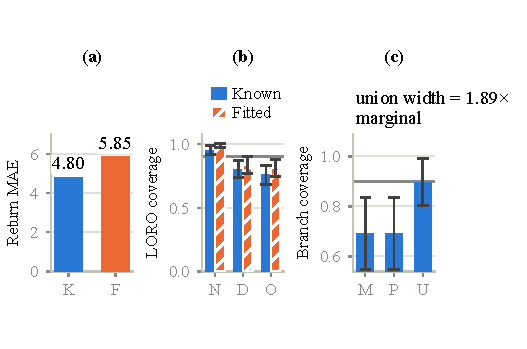
\includegraphics[width=0.55\linewidth]{../../figures/scis/fig7-general-pomdp.pdf}
\caption{Second synthetic sensor-POMDP testbed. K/F denote Known/Fitted (identified/fitted) transition. Panel (a), return-prediction MAE. Panel (b), raw leave-one-regime-out coverage by regime. Panel (c), identified-transition raw intervention-branch coverage under marginal, pre-decision, and branch-union calibration; panels (b) and (c) error bars are 95\% binomial intervals. Gray lines mark nominal 0.90 coverage; the gray annotation in panel (c) gives the branch-union width relative to the marginal width (1.89$\times$). x-axis codes: K/F = Known/Fitted, N/D/O = normal/degraded/outage, M/P/U = marginal/pre-decision/branch-union.}
\label{fig:7}
\end{figure}

\subsection{Observation-map identification (L3)}

The observable-only procedure recovers \texttt{stale\_phi}, \texttt{stale\_sd}, and \texttt{ext\_sd} close to their generating values, but \texttt{open\_sd} and \texttt{ext\_phi} remain weakly identified. The main \texttt{ext\_phi} estimate is 0.7741 (truth 0.8), with a 90\% bootstrap interval [0.7480, 0.7930]; trimming moves the estimate from 0.7481 to 0.8455. Because the threshold is chosen, this is a specification-specific interval, not a uniform confidence statement.

Coverage is nevertheless stable across the true-$S$ G0 diagnostic and four observable $h$ specifications: pooled $G$ varies by at most 0.6 pp for Wide and 0.4 pp for Narrow, and the largest per-regime spread is 2.7 pp. The coverage conclusions therefore do not depend on treating \texttt{h\_obs} as truth, although the weakly identified parameters remain a boundary. Figure~\ref{fig:6} and Appendix Table B13 give the full specification curve.

\begin{figure}[!ht]
\centering
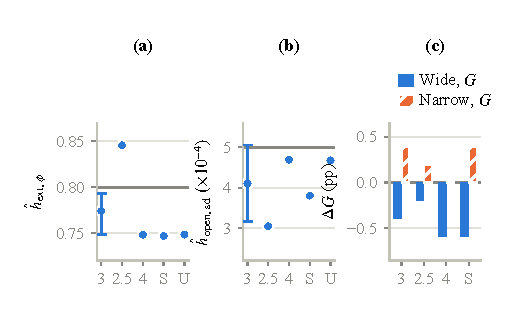
\includegraphics[width=0.55\linewidth]{../../figures/scis/fig6-l3-h.pdf}
\caption{Panels (a) and (b) vary the $h$ specification; dots are point estimates, the whisker on the main row is the 90\% bootstrap interval, and the gray line is the simulator truth. These $h$ estimates are common to both the Wide and Narrow policies (the Wide/Narrow legend applies only to panel (c)). Panel (c) is the change in $G$ coverage relative to the true-$S$ G0 row (percentage points); nominal coverage is 90\% ($\alpha=0.1$), and no 95\% interval is attached to individual cells. x-axis codes: 3/2.5/4 = trim threshold $z$, S = OPEN-sd volatility, U = unmasked MLE.}
\label{fig:6}
\end{figure}

\subsection{Stress and misspecification robustness}

The unfreeze-jump stress variant produces the failure described by Theorem 4. With $\gamma_{\mathrm{st}}=4$, open-only calibration covers 0.864 (oracle) and 0.843 (estimated), whereas cross-event calibration reaches 0.902 and 0.902 at 1.10$\times$ and 1.16$\times$ width. The $\gamma_{\mathrm{st}}=0$ placebo gives 0.906/0.895 and 0.901/0.900, with no false positive. The OPEN-to-OPEN one-step kernel is $\gamma_{\mathrm{st}}$-free by construction, whereas the de-freeze $z^2$ variance ratio is 1.233 with paired path-permutation $p=0.0005$: the signal is cross-event variation, not open increments.

The full stress-test table is provided in the supplementary material.

\textbf{Non-Markov bridge.} Appendix Table B2 replaces the jump with the bridge law of Theorem 4. In the $\nu_{\rm mult}=0.6$ world, open-only calibration covers 0.818 (oracle) and 0.806 (estimated), while cross-event calibration reaches 0.900 and 0.900 at 1.27$\times$ and 1.32$\times$ width. Same-endpoint observed paths remain bit-identical under $\nu$ and $2\nu$ despite a latent QV ratio of 3.85. Cross-event calibration therefore recovers marginal coverage, not coverage conditional on the latent bridge state.

\textbf{Misspecification suite.} Appendix Table B4 perturbs observation-noise memory, jump tails, regime labels, and a hidden stale state. Identified bias stays within absolute value 0.0053, and identified plug-in $G$ coverage stays at 0.822--0.861 against 0.621--0.723 naive. In contrast, the conformal component is fragile: full-window differences are not uniformly positive, regime-label noise removes the small identified CQR edge, and no perturbation repairs LORO coverage (identified 0.861--0.875, naive 0.872--0.884). Thus identification robustly helps bias and plug-in coverage, but conformal recovery requires trustworthy regime labels and does not remove the LORO boundary.

The suite uses one perturbation magnitude per class and the same 128+128 seeds, so it supports these four departures rather than a dose-response map.

\subsection{Semi-synthetic calibration}

The semi-synthetic calibration anchors scales rather than reproducing a market. Mean reversion and jump frequency bracket the simulator, while its volatility is deliberately at the high end. Measured weekend and holiday gap sd is 0.26--0.40 of the continuous-diffusion scale and 0.54--0.95 of the $\gamma_{\mathrm{st}}=4$ jump-only scale, so the stress is conservative relative to the four feeds. This does not independently validate $h$, the exact freeze duration, or the policy family; it establishes that the synthetic scales are of the right order.

\subsection{Real-path usage check in a liquid-regime case}

This \textbf{post-hoc, regime-conditional case} tests the pipeline on observed pool paths. After inspecting month-level liveness, we selected the 2026-07-01 to 2026-10-20 liquid-regime window and replayed two target policies on 33 of 48 candidate A-layer events (68.8\%) in three Ethereum Ondo pools. The events span 16 independent freeze episodes (15 TSLA, 15 SPY, 3 NVDA), with 16 economically thin and 17 non-thin. The larger nine-month audit fails the pre-registered G1-R availability gate, so this is a replayable liquid-regime subset, not a representative market sample.

\textbf{Data and protocol.} Truth is deterministic target-policy replay with P-marked fee income, change in IL at the observed price, and gas/slippage costs. One observed realization identifies neither a deployed-policy counterfactual nor price impact. The identified pipeline uses regime-dependent volatility and a stale anchor; the naive pipeline treats the observed price as a random walk. We use leave-one-freeze-episode-out split conformal at $\alpha=0.1$, with raw, studentized, and CQR scores plus a plug-in normal benchmark. Observation-map parameters are estimated once on all events; episode folds recalibrate only the conformal radius. Full data and model specifications are in Appendix Tables B9A--B9C.

\textbf{Coverage and width.} At nominal 0.9, both pipelines cover 30/33 (0.909) on all five targets. At equal coverage, the identified freeze interval is $3.30\times10^{-4}$ wide versus $1.91\times10^{-3}$ naive (ratio 0.17), with 7.8$\times$ lower MAE. Aggregate event intervals are not sharper: width is $4.02\times10^{-3}$ versus $4.14\times10^{-3}$ (ratio 0.97), and identified MAE is $1.05\times10^{-3}$ versus $0.96\times10^{-3}$ naive. The observation map therefore buys sharpness where the drift is, not uniformly. The three uncovered total-window events are all TSLA; identified covers all four holiday freeze events versus two of four naive.

\textbf{Branch diagnostics.} The Wide policy has only 7 of 33 post-open rebalances, below the nine calibration events needed for a finite 90\% branch interval, so its union interval is not identifiable. The Narrow policy has 14 of 33; its union interval covers 0.970 at 1.28$\times$ the marginal width. This mirrors the width/power trade-off in \S5.2.

\textbf{Transfer diagnostics.} Raw leave-one-symbol-out coverage on TSLA is 0.267 for both pipelines because its fee tier and volatility put its reward scale outside the SPY/NVDA calibration. CQR repairs it to 0.933 for both; within-symbol calibration also gives 0.933 macro coverage over SPY and TSLA, while NVDA's three events are too few for a 90\% radius. The in-sample 2h$\to$24h shift gives 0.879 identified and 0.848 naive. Thus a pooled radius is neither a cross-symbol nor a per-symbol duration guarantee; the fold counts do not identify the cause of failure.

\textbf{Window sensitivity.} A nine-month rerun over 53 replayable events and 32 freeze episodes retains 48/53 pooled coverage (0.906) and the freeze-width advantage. It also exposes calibration-window dependence: identified total-window coverage is 17/22 on SPY, 27/27 on TSLA, and 4/4 on NVDA; the post-open width ratio reverses to 1.22. The in-sample 2h$\to$24h shift falls to 0.415 identified versus 0.792 naive, with identified coverage of 1/22 on SPY, 17/27 on TSLA, and 4/4 on NVDA. We therefore treat transfer, thin-event, and width results as diagnostics of the calibration window rather than stable advantages.

\textbf{Caveats.} The main case has only three NVDA events, and truth is single-path, model-based replay. The observation map is fit once on all events rather than nested cross-validation. Interpretation is limited to this regime-conditional usage case, not a representative market study or causal deployed-policy evaluation.

\subsection{Answers to Q1--Q3}

Q1 (Theorem 1; L3 results): the observation kernels, short-range dynamics, belief, and value are identified under the stated assumptions, with I5/I5$'$ required only for the non-Markov bridge; \texttt{open\_sd} and \texttt{ext\_phi} remain weakly identified. Q2 (L0--L2 and second synthetic testbed; \S5.2, \S\S7.1--7.4; Appendix Table B7): evaluation-regime calibration recovers marginal coverage, while calibration-side branch labels recover branch coverage at a width price; LORO remains a boundary, and the conformal identified-versus-naive gain is fragile to regime-label noise. Q3 (Theorems 3 and 4): pre-decision information cannot guarantee post-decision branch coverage for branch-blind, nondegenerate score rules, and observationally equivalent non-Markov models can differ in value when endpoints do not determine the bridge reward (Appendix Table B8); Appendix Table B1 retains all three decomposition terms rather than a uniform value-error bound.

\section{Discussion and limitations}

\subsection{Implications for practice}

Protocol 1 turns the boundary map into a reusable audit that separates recoverable coverage from missing support and information limits.

\small
\noindent\textbf{Protocol 1: Regime-aware OPE coverage audit.}
\textbf{Input.} Logged trajectories $\{(P_t,a_t,r_t)\}$ with timestamps and calendar labels; target policy $\pi$; nominal level $1-\alpha$; a calibration/evaluation split; candidate observation maps $h_r$.

\begin{enumerate}
\item \textbf{Support.} State whether the window was pre-registered; if post-hoc, label the result descriptive. Tabulate calibration/evaluation events by regime and symbol; pre-specify $n_{\min}$; mark under-supported regimes and omit their regime-conditional claims. Report leave-one-regime-out coverage per regime.
\item \textbf{Observation map.} State which components of $h_r$ are estimated and which are fixed; report a specification curve over weakly identified components (in this paper, \texttt{open\_sd}, \texttt{ext\_phi}, trimming). If coverage moves, report the range, not a single plug-in value.
\item \textbf{Coverage and branch timing.} Report L0 (row), L1 (trajectory), and L2 (branch) separately, with $n$, coverage, a 95\% interval, and width; flag small cells (this paper uses $n\leq 24$) as directional. If the branch label is not in the pre-decision $\sigma$-field, branch-wise calibration needs calibration-side labels and pays a width price (Proposition 2); report the branch gap and width ratio.
\item \textbf{Identification and report.} For a non-Markov bridge, check cross-event variation; the identification level is reported when variation is absent. Report the level achieved, calibration support, coverage/width, branch gaps, and the $h$ range.
\end{enumerate}

\textit{Stop rules.} Stop and report a negative result if L0 fails, a regime is unsupported, branch coverage is claimed without branch labels, or a non-Markov bridge lacks cross-event variation. Do not repair a failed level by pooling.
\normalsize

Protocol 1 makes the achieved level, calibration support, and width inseparable. The levels are diagnostic, not ordered by repair difficulty: passing L0 does not imply L1 or L2.

\subsection{Limitations}

\textbf{1. Controlled evidence and identification scope.}

The controlled synthetic environment shares the latent law across regimes and changes only the observation kernel; fees, maximal extractable value (MEV), oracle latency, and cross-venue basis are absent, so it isolates the observation map rather than live-market magnitudes. In the general sensor-POMDP, the identified-transition predictor is treated as the target setup, while the fitted-transition comparator estimates only its rollout transition; the shared observation filter means this is not an observation-filter ablation or a joint-estimation study. The dynamics parameters $\kappa$, $\mu$, and the jump law are fixed, and $\sigma$ is known in the main experiments; only $h$ is estimated, and joint estimation is not tested. Moreover, \texttt{ext\_phi} is weakly identified in this design and trimming range. Theorem 1 and its positive results are within-family identification statements; the misspecification suite (\S7.6) probes one perturbation per class, and the conformal identified-vs-naive gain does not survive regime-label noise while the bias and plug-in components do survive.

\needspace{3\baselineskip}
\textbf{2. Estimation-side uncertainty and calibration scope.}

Uncertainty in $h$ is not propagated through a joint sampling distribution: L3 varies $h$ after the fact, so the resulting coverage stability is a robustness observation rather than a corollary of Theorem 1(e). The calendar is shared across calibration and test, so LORO measures regime-shift robustness rather than extrapolation to a future calendar; regime-aware calibration repairs marginal coverage only when evaluation-regime calibration data exist and does not repair all observation-map drift. Logging policies are heuristic, and standard observed-reward IPS/DR are unavailable because the reward contains an unobserved path functional; comparisons are plug-in versus conformal rather than among OPE estimators. The branch-union bound is sufficient, not optimal; the post-rebalance branch is unavailable at prediction time; branch-wise calibration needs calibration-side labels; and the trivial bound can be loose.

\textbf{3. Real-path scope.}

The real-path case is a post-hoc, model-based, calibration-window-specific usage check rather than a representative market study or a causal deployed-policy evaluation: Section 7.8 reports its sample and model boundaries and the nine-month sensitivity. Synthetic conclusions are therefore limited to the controlled evidence; a larger pre-registered empirical study is required before transfer to live tokenized equities.



\section{Conclusion}\label{sec:conclusion}

Theorem 1 identifies value under its assumptions, with I5/I5$'$ for non-Markov bridges. Branch-blind marginal coverage does not identify branch coverage; calibration-side labels restore it at a width price. Observationally equivalent non-Markov models can differ in value. Protocol 1 reports support, observation-map uncertainty, coverage, width, and information limits; the real-path case remains a usage check.



\Acknowledgements{This work was supported by the Science and Technology Projects of Xizang Autonomous Region\protect\\ (Grant No. XZ202501ZY0060).}
\Supplements{Appendixes A--F.}
\DeclarationofAI{During the preparation of this manuscript, the authors used Kimi Code CLI 2.5.2--2.5.3 (K3.1-Pro) for language polishing, grammar checking, and code assistance. The authors manually verified the AI-generated content and take full responsibility for the accuracy, completeness, and originality of the entire manuscript.}

\bibliographystyle{scis}
\bibliography{refs}

\end{document}
